%TODO: add cliffhanger with preview for next time
%TODO: add learning outcome slide
%TODO: shorten team work+move earlier

% Make nice A4 pages for print:
%\usepackage{pgfpages}
%\pgfpagesuselayout{resize to}[a4paper,border shrink=5mm,landscape]

\beamertemplatenavigationsymbolsempty

\setbeamertemplate{bibliography item}[text]

\usepackage[type={CC},modifier={by-sa},version={4.0}]{doclicense}

\usepackage[utf8]{inputenc}
\usepackage{hyperref}
\usepackage{breakurl}
\usepackage{graphicx}
\usepackage{pgfplots}
\usepackage{pgf}
\usepackage{tikz}
\usetikzlibrary{positioning}
\usetikzlibrary{arrows}
\usetikzlibrary{decorations.markings}
\usetikzlibrary{calc}
\usetikzlibrary{matrix}
\usetikzlibrary{shapes}
\usetikzlibrary{decorations.pathmorphing}
\usetikzlibrary{fit}
\usetikzlibrary{backgrounds}
\usetikzlibrary{plotmarks}
\usepackage{stmaryrd}
\usepackage{listings}
\usepackage{pdflscape}
\usepackage{perpage}
\usepackage{appendixnumberbeamer}

%\usepackage[thmmarks,amsmath,amsthm]{ntheorem} % already included in beamer
\usepackage{thm-restate}

\usepackage[sort&compress,numbers]{natbib}  % to be have \citet, \citeauthor, \citeyear

\MakePerPage{footnote}

\tikzstyle{o}=[r,ppBlue]
\tikzstyle{r}=[thick,rectangle,align=center]
\tikzstyle{t}=[r,ppTrans] %,font=\bfseries]
\tikzstyle{dd}=[densely dashed]
\tikzstyle{n}=[r,ppBlue]
\tikzstyle{p}=[r,ppRed]
\tikzstyle{ppRed}  =[draw=red,  fill=  red!20]
\tikzstyle{ppBlue} =[draw=blue, fill= blue!20]
\tikzstyle{ppGreen}=[draw=green,fill=green!20]
\tikzstyle{ppTrans}=[draw=none, fill=none]

\usetheme{Warsaw}

\useoutertheme[subsection=true]{smoothbars}
%\useoutertheme[subsection=false]{miniframes}

\definecolor{bblue}{HTML}{D7DF01}	% yellow-ish actually, for better black/white printing
\definecolor{rred}{HTML}{C0504D}
\definecolor{ggreen}{HTML}{9BBB59}
\definecolor{ppurple}{HTML}{9F4C7C}
\definecolor{lightgray}{rgb}{0.3,0.3,0.3}
\definecolor{lightergray}{rgb}{0.9,0.9,0.9}
\definecolor{UniBlue}{RGB}{83,121,170}

\DeclareTextFontCommand\textintro{\normalfont\bfseries\itshape} % nice!
\newcommand{\intro}[2][]
{%
	\textintro{#2}%
}
\newcommand{\empha}[2][]
{%
	\emph{#2}%
}

%\theoremstyle{plain}
\newcounter{reqcounter}
\newtheorem{requirement}[reqcounter]{Requirement}

%setbeamercolor{structure}{fg=violet}

\makeatletter
\def\th@task{%
    \normalfont % body font
    \setbeamercolor{block title example}{bg=orange,fg=white}
    \setbeamercolor{block body example}{bg=orange!20,fg=black}
    \def\inserttheoremblockenv{exampleblock}
  }
\makeatother

\theoremstyle{task}
\newtheorem{task}{Task}

\newenvironment{assignment}%
{%\setbeamercolor{background canvas}{bg=violet}%
%\setbeamercolor{structure}{fg=cyan!90!black}%
 \setbeamercolor{frametitle}{bg=orange,fg=white}
\begin{frame}}%
{\end{frame}}%

\AtBeginSection[]{
  \begin{frame}
  \vfill
  \centering
  \begin{beamercolorbox}[sep=8pt,center,shadow=true,rounded=true]{title}
    \usebeamerfont{title}\insertsectionhead\par%
  \end{beamercolorbox}
  \tableofcontents
  \vfill
  \end{frame}
}




\pgfplotsset{compat=1.14}
\author{Markus Raab}


\date{22.05.2019}

\begin{document}

\renewcommand{\enquote}[1]{\emph{``#1''}} % Cannot be done earlier

%%%%%%%%%%%%%%%%%%%%%%%%%%%%%%%
\begin{frame}
	\titlepage
	\doclicenseThis
\end{frame}

\begin{frame}
	Lecture is every week Wednesday 09:00 - 11:00.

	\begin{description}
		\item[06.03.2019:] {\color{gray}topic, teams}
		\item[13.03.2019:] {\color{gray}TISS registration, initial PR}
		\item[20.03.2019:] {\color{gray}other registrations, guest lecture}
		\item[27.03.2019:] {\color{gray}PR for first issue done, second started}
		\item[03.04.2019:] {\color{gray}first issue done, PR for second}
		\item[10.04.2019:] {\color{gray}mid-term submission of exercises}
		\item[08.05.2019:] {\color{gray}different location: Complang Libary}
		\item[15.05.2019:]
		\item[22.05.2019:] {\color{red}all 5 issues done}
		\item[29.05.2019:]
		\item[05.06.2019:] final submission of exercises
		\item[12.06.2019:]
		\item[19.06.2019:] last corrections of exercises
		\item[26.06.2019:] exam
	\end{description}
\end{frame}

\begin{assignment}
	\frametitle{Tasks for today}
	(until 22.05.2019 23:59)

	\begin{task}
	All issues done.
	\end{task}
\end{assignment}

\begin{assignment}
	\frametitle{Tasks for next week}
	(until 29.05.2019 23:59)

	\begin{task}
	Continue teamwork and homework.
	\end{task}
\end{assignment}

\begin{frame}
	\frametitle{Popular Topics}
	\vspace{-0.55cm}
	\setlength{\columnsep}{-1.3cm}
	\raggedright
	\definecolor{amethyst}{rgb}{0.6, 0.4, 0.8}
	\begin{multicols}{2}
	\begin{description}
	\item[14] {\color{orange} tools}
	\item[9] {\color{amethyst} testability}
	\item[9] {\color{gray} code-generation}
	\item[7] context-awareness
	\item[6] {\color{red} specification}
	\item[6] misconfiguration
	\item[6] {\color{gray} complexity reduction}
	\item[5] validation
	\item[5] {\color{amethyst} points in time} % (early detection)
	\item[5] error messages
	\item[5] {\color{gray} auto-detection}
	\item[4] user interface
	\item[4] {\color{red} introspection}
	\item[4] design
	\item[4] cascading
	\item[4] {\color{amethyst} architecture of access}
	\item[3] {\color{gray} configuration sources}
	\item[3] {\color{gray} config-less systems}
	\item[2] secure conf
	\item[2] {\color{gray} architectural decisions}
	\item[1] push vs.\ pull
	\item[1] infrastructure as code
	\item[1] full vs.\ partial
	\item[1] convention over conf %iguration
	\item[1] CI/CD
	\item[0] {\color{red} documentation}
	\end{description}
	\end{multicols}
\end{frame}



\begin{frame}
	\frametitle{Goals for today}
	\textit{learning outcome:}
	\begin{itemize}
	\item remember how to use configuration specification as documentation
	\item remember requirement for synchronization
	\item remember example of 3-way merge
	\item remember types of configuration
	\item being able to design and architect a configurable software application
	\end{itemize}
\end{frame}








\begin{frame}
	\frametitle{Modularity (Recapitulation)}
	\pause
	\Large
	\ExecuteMetaData[../book/backend.tex]{definition-modularity}
\end{frame}


\begin{frame}
	\frametitle{Introspection (Recapitulation)}
	\begin{task}
	What is internal and external specification?
	What is introspection?
	\end{task}

	\pause
	\vspace{1em}

	\begin{itemize}
	\item internal: within applications' source code
	\item unified get/set access to (meta*)-key/values
	\item access via applications, CLI, GUI, web-UI, ...
	\item access via any programming language (similar to file systems)
	\item GUI, web-UI can semantically interpret metadata
	\item needed as communication of producers and consumers of configuration
	\item essential for \intro[no-futz computing]{no-futz computing}~\citet{holland2001nofutz}
	\end{itemize}
\end{frame}

\begin{frame}
	\frametitle{Guarantees (Recapitulation)}
	\begin{alertblock}{Question}
	How to ensure that configuration access points match with present configuration settings?
	\end{alertblock}

	\pause
	\vspace{1em}

	\textbf{Configuration Specification}:
	\begin{itemize}
	\item without specification you and others do not even know which settings are available
	\item needed for any further techniques we will discuss:
		\begin{itemize}
		\item code generation guarantees that configuration access points match with specification
		\item validation guarantees that configuration settings match with specification
		\end{itemize}
	\end{itemize}
\end{frame}


\begin{frame}
	\frametitle{Testing (Recapitulation)}
	\begin{alertblock}{Question}
	What do we want to test?
	What do we ask ourselves?
	\end{alertblock}

	\pause

	\begin{itemize}
	\item That settings do what they should (devs and admins)
	\item That settings are properly validated (devs~\cite{xu2013blame})
	\item Regression tests~\cite{qu2008configuration}
	\vspace{1em}
	\item Are all settings implemented?
	\item Are all settings used in tests?
	\item Are there unused settings in the code?
	\end{itemize}
\end{frame}

\begin{frame}
	\frametitle{When are settings used? (Recapitulation)}

	\pause

	\begin{description}[<+-| alert@+>]
	\item[Implementation-time] configuration accesses \index{implementation-time}
	are hard-coded settings in the sou\-rce code repository.
	For example, architectural decisions~\cite{zdun2007patterns} lead to impl\-ementation-time settings.

	\item[Compile-time] configuration accesses \index{compile-time}
	are configuration accesses resolved by the build system while compiling the code.

	\item[Deployment-time] configuration accesses \index{deployment-time}
	are configuration accesses while the software is installed.

	\item[Load-time] configuration accesses \index{load-time}
	are configuration accesses during the start of applications.

	\item[Run-time] configuration accesses \index{run-time}
	are configuration accesses during execution not limited to the startup procedure.
	\end{description}
\end{frame}

\begin{frame}
	\frametitle{Latent Misconfiguration (Recapitulation)}
	Phases when we can detect misconfigurations:
	\begin{itemize}[<+-| alert@+>]
	\item Compilation stage in configuration management tool
	\item Writing configuration settings on nodes
	\item Starting applications (load-time)
	\item When configuration setting is actually used (run-time)
	\end{itemize}

	\pause[\thebeamerpauses]

	\begin{alertblock}{Problem}
	More context vs. easier to detect and fix.
	\end{alertblock}
\end{frame}














%%%%%%%%%%%%%%%%%%%%%%%%%%%%%%%%%%%%%%%%%% 
\section{Documentation}

\subsection{}


\begin{frame}
	\ExecuteMetaData[../book/motivation.tex]{documentation-inform}
\end{frame}

\begin{frame}
	There are at least two forms of documentation necessary:

	\begin{itemize}
	\item Explanations
	\item Examples
	\end{itemize}

	Generation helps to avoid duplication:

	\ExecuteMetaData[../book/motivation.tex]{documentation-req}
\end{frame}

\begin{frame}
	\begin{alertblock}{Question}
	How to avoid duplication between description text and other parts?
	\end{alertblock}

	\pause

	\begin{itemize}
	\item Render type and defaults into the documentation
	\item Render requirements and rationale into the documentation
	\item Use visibility to only show relevant configuration settings
	\end{itemize}
\end{frame}

\begin{frame}[fragile]
	\frametitle{Example}

	\begin{code}[gobble=4]
	[slapd/threads/listener]
	  check/range:=1,2,4,8,16
	  default:=1
	  description:=adjust to use more threads
	  rationale:=needed for many-core systems
	  requirement:=1234
	  visibility:=user
	\end{code}
\end{frame}

\begin{frame}
	\frametitle{Reevaluate specifications (Recapitulation)}

	In which situations should you reevaluate if a configuration setting (specification) is needed?

	\pause

	\ExecuteMetaData[../book/implications.tex]{reasons-adding}
\end{frame}


%%%%%%%%%%%%%%%%%%%%%%%%%%%%%%%%%%%%%%%%%% 
\section{3-way merge}

\subsection{}

\begin{frame}
	\frametitle{Synchronization}

	Problem: transient and persistent configuration settings might be out-of-sync~\cite{jin2014configurations}

	\pause

	\ExecuteMetaData[../book/motivation.tex]{req-consistency}

	\pause

	Solutions:
	\begin{itemize}
	\item Often write out configuration settings.
	\end{itemize}
\end{frame}

\begin{frame}
	\frametitle{Semantic 3-way merge}

	Problem: When trying to writing out configuration settings, the configuration settings might not be as they were before. (Conflict)

	\pause

	Solution: Many conflicts can be resolved automatically with a semantic 3-way merge.

	\pause

	We can resolve many conflicts automatically if we consider:
	\begin{itemize}[<+-| alert@+>]
	\item the key/value structure (vs. line-based)
	\item the origin of the configuration settings
	\item the type of settings
	\end{itemize}

	\pause[\thebeamerpauses]

	For example, when upgrading slapd:
	\begin{itemize}
	\item System administrator changed the file (Ours).
	\item Package maintainer changed the file (Theirs).
	\end{itemize}
\end{frame}

\begin{frame}[fragile]
	\frametitle{Conflicts Example}

	\textbf{Ours:}
	\begin{code}[gobble=4,language=CfgElektra]
	slapd/threads/listener=4

	slapd/threads/enable= \
		yes # must be enabled for listener

	\end{code}

	\textbf{Theirs:}
	\begin{code}[gobble=4,language=CfgElektra]
	slapd/threads/enable = on
	slapd/threads/listener = 8
	\end{code}

	\pause
	\textbf{Origin:}
	\begin{code}[gobble=4,language=CfgElektra]
	slapd/threads/listener=8
	slapd/threads/enable = true
	\end{code}
\end{frame}





%%%%%%%%%%%%%%%%%%%%%%%%%%%%%%%%%%%%%%%%%% 
\section{Team Work}

\subsection{}

\begin{frame}
	\frametitle{Steps}


	\begin{enumerate}
	\item Familiarize yourself with the description of the proposed configuration system. (5 min)
	\item Find a group and decide who will create flip chart, moderate, and present. (1 min)
	\item Give yourselves roles (admin, dev, user) and split the goals among them. (1 min)
	\item Create together an architecture that fulfils the goals. (ca.~40~min)
	\item Present that architecture. (5 min)
	\end{enumerate}
\end{frame}

\begin{frame}
	\frametitle{Goals}

	\begin{enumerate}
	\item configuration-management friendly
	\item early detection of misconfiguration
	\item transient and persistent configuration consistent
	\item correct documentation
	\item reuse software as much as possible but integrate them nicely
	\end{enumerate}
\end{frame}

\begin{frame}
	\frametitle{Requirements}

	Design a camera system:

	\begin{enumerate}
	\item that is able to take single pictures and streams
	\item pluggable camera modules (lenses, image sensor, ...)
	\item should have camera profiles for different vendors
	\item a Web-UI that shows all configuration settings
	\item support yet-unknown remote configuration protocol\linebreak(Web, SNMP, CMs, ...)
	\end{enumerate}
\end{frame}

\begin{frame}
	\frametitle{Tasks}

	\begin{enumerate}
	\item design the architecture of configuration settings
	\item design the architecture of configuration access
	\item design how the CM tools should look like
	\item tracer bullet~\cite{hunt1999pragmatic}: explain for one configuration setting the whole way from source to destination
	\item make decisions (which languages, which software, how to achieve the goals)
	\item explain how to ensure smooth configuration upgrades
	\item explain how to provide documentation for operators
	\item explain how to reuse software
	\end{enumerate}
\end{frame}








%%%%%%%%%%%%%%%%%%%%%%%%%%%%%%%%%%%%%%%%%% 
\section{Context-Awareness}

\subsection{}

\begin{frame}
	If you're a baker, making bread, you're a baker. If you make the best bread in the world, you're not an artist, but if you bake the bread in the gallery, you're an artist. So the context makes the difference.\par\raggedleft--- \textup{Marina Abramovic}
\end{frame}

\begin{frame}
	\ExecuteMetaData[../book/background.tex]{context-definition}
\end{frame}

\begin{frame}
	\frametitle{Types of Configuration}
	\begin{description}
	\ExecuteMetaData[../book/background.tex]{context-types}
	\end{description}
\end{frame}

\begin{frame}
	\hspace*{-1em}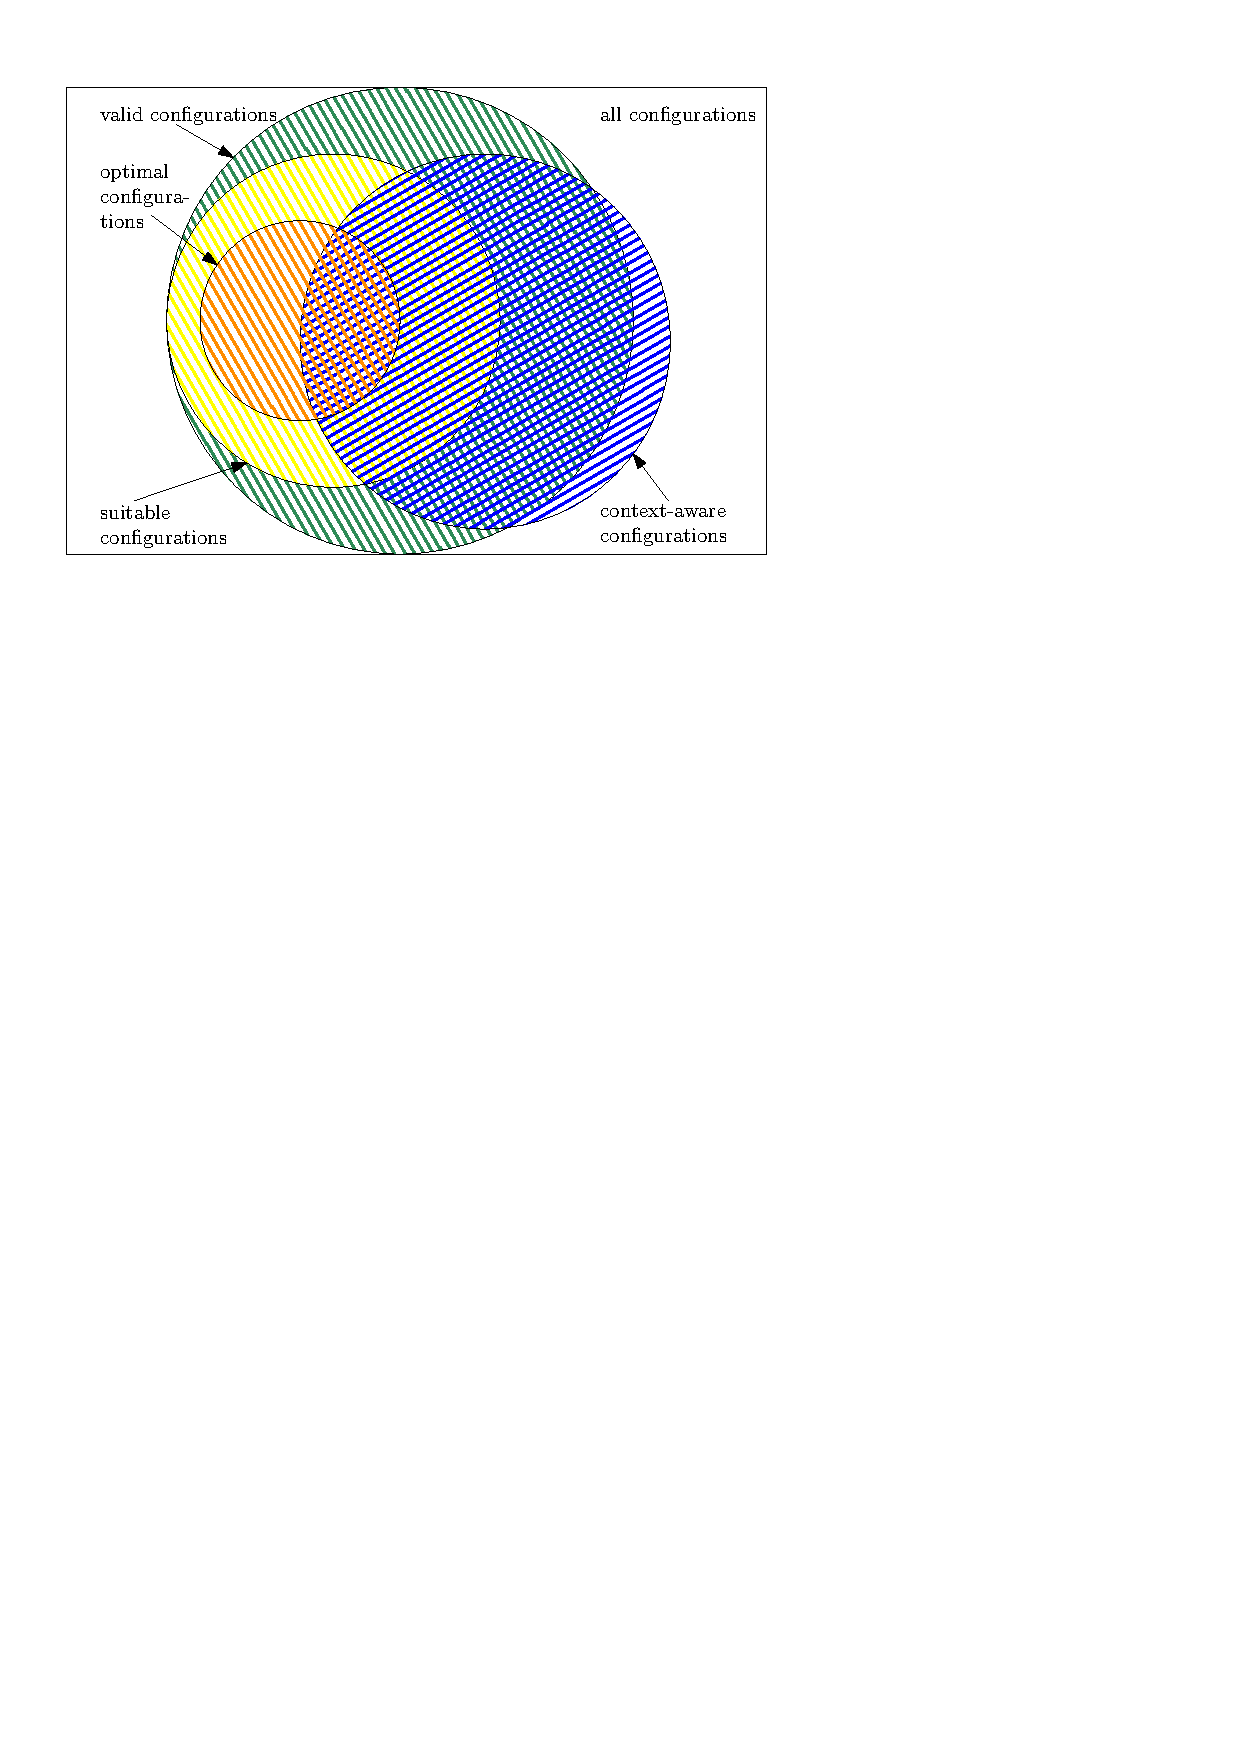
\includegraphics{configurations}
\end{frame}

\begin{frame}
	\frametitle{Viewpoints}
	\begin{description}
	\item[Sensors:] derive context from information sources of the system.
	Adding new context sensors increases the context available in a system.
	\ExecuteMetaData[../book/background.tex]{context-viewpoints}
	\end{description}
\end{frame}

\begin{frame}
	\frametitle{Cascading (Recapitulation)}
	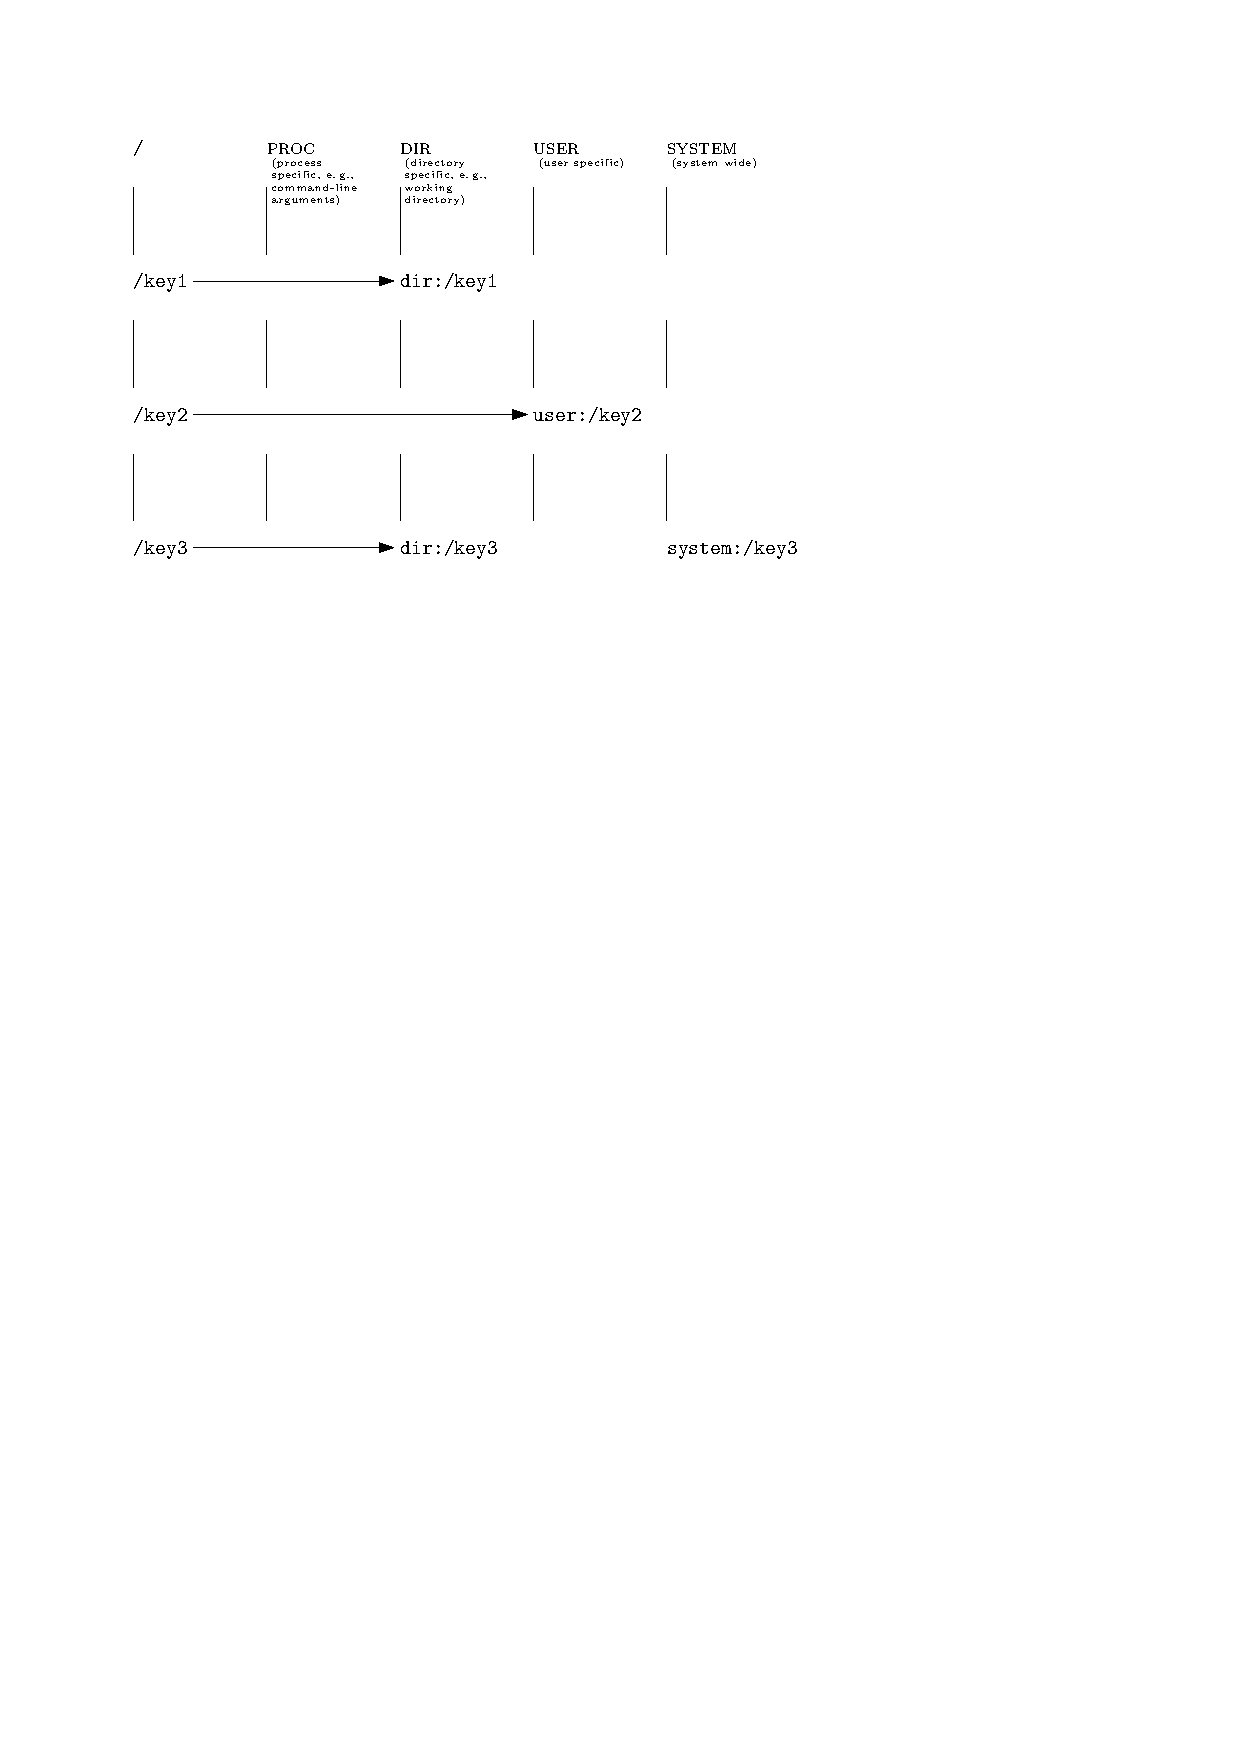
\includegraphics{cascading}
\end{frame}

\begin{frame}[fragile]
	\frametitle{Context-aware Lookup}

	\begin{itemize}
	\item
	Determine threads from CPUs:

	\begin{code}[gobble=4]
	[env/layer/cpu]
	  type:=long
	[slapd/threads/listener]
	  context:=/slapd/threads/%cpu%/listener
	\end{code}

	\item
	Determine vibration from sensors:

	\begin{code}[gobble=4]
	[phone/call/vibration]
	  type:=boolean
	  context:=/phone/call/%inpocket%/vibration
	\end{code}

	\item
	Determine proxy settings from network:

	\begin{code}[gobble=4]
	[env/override/http_proxy]
	  context:=/http_proxy/%interface%/%network%
	\end{code}
	\end{itemize}
\end{frame}







%%%%%%%%%%%%%%%%%%%%%%%%%%%%%%%%%%%%%%%%%% 
\nocite{raab2017introducing}

\appendix

\begin{frame}[allowframebreaks]
	\bibliographystyle{plainnat}
	\bibliography{../shared/elektra.bib}
\end{frame}

\end{document}


%TODO: add cliffhanger with preview for next time
